\chapter{Volatility Modeling}
\label{chap:2}

The objective of this chapter is to introduce econometric methods commonly used to model the conditional volatility of asset returns, $\sigma_{t+1}$. These models are collectively referred to as conditional heteroscedastic models.

As noted by \citeA{Tsay2010}, a distinctive feature of stock volatility is that it is not directly observable. Daily volatility cannot be directly inferred from return data because there is only one observation per trading day. However, despite its unobservability, volatility exhibits certain characteristics that are consistently observed in asset returns.

First, as established in the previous chapter, volatility—measured by squared returns—exhibits strong autocorrelation. This implies that if a recent period experienced high variance, the following day is also likely to exhibit high variance, forming what are known as volatility clusters. Figure~\ref{2.1} shows the squared S\&P 500 returns used previously. Observe that volatility is not constant and exhibits distinct clustering patterns.

\begin{figure}[H]
    \centering
    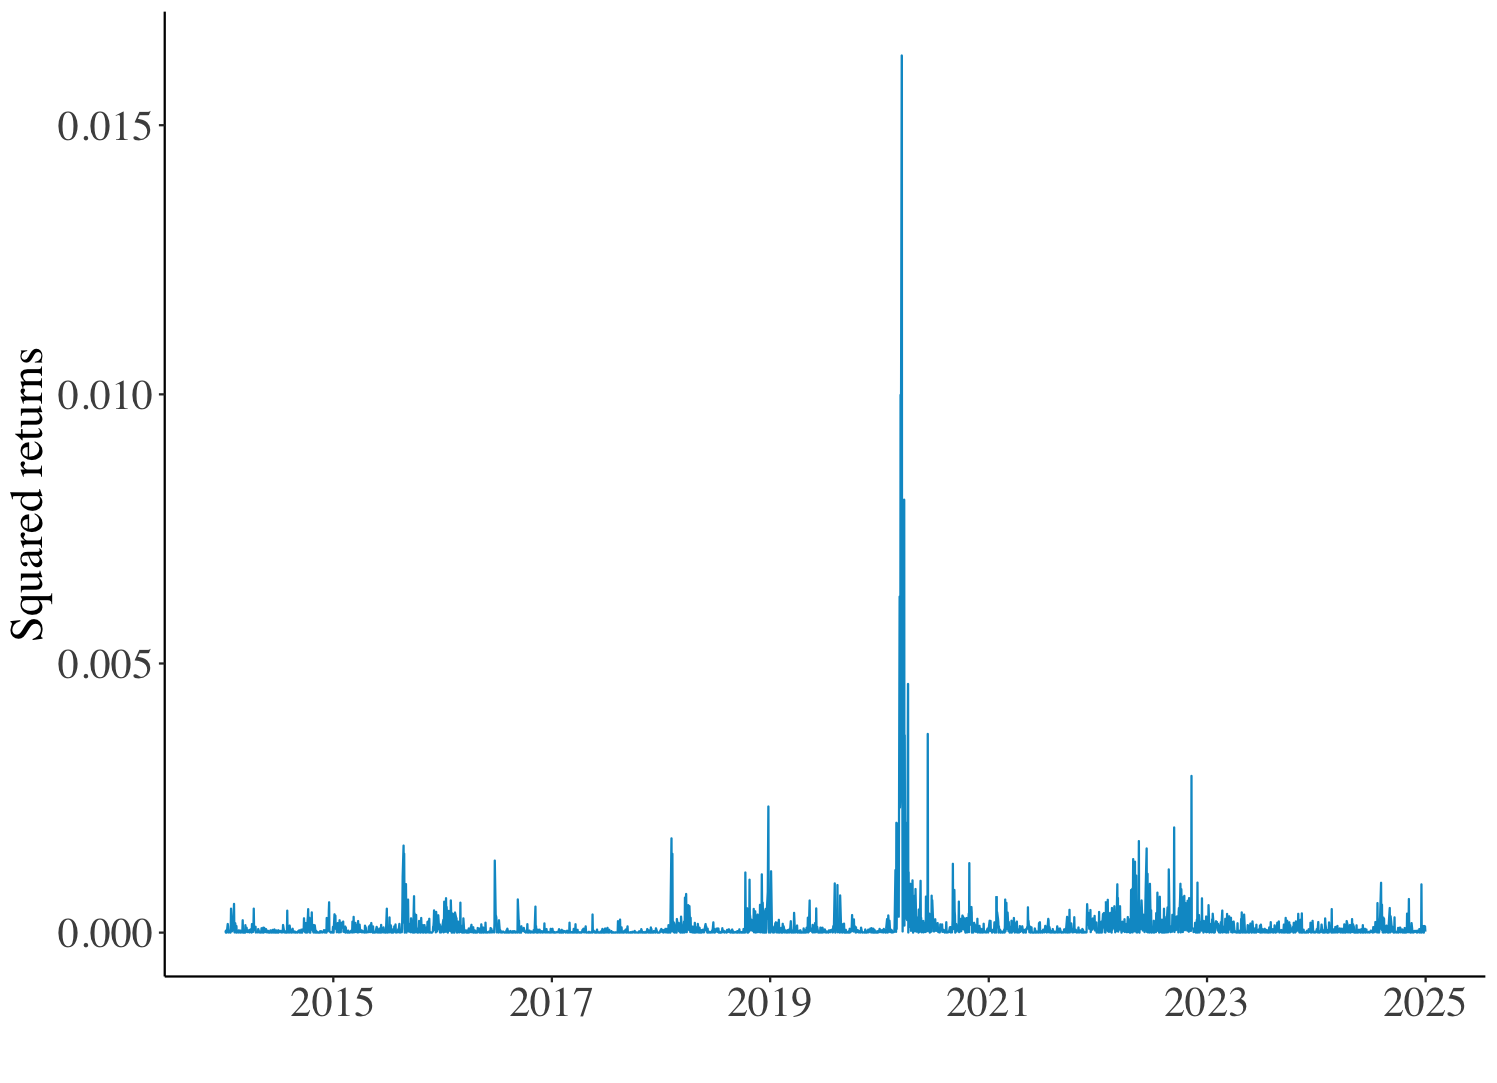
\includegraphics[scale=0.18]{../../plots/2.1.png} % Replace 
    \caption{Squared S\&P 500 returns, 2014-2024.}
    \label{2.1}
\end{figure}

Additionally, volatility evolves continuously over time, does not diverge to infinity, and, as previously discussed, appears to respond asymmetrically to large price increases and decreases.

The literature on volatility models is extensive. Early models were developed to capture the dynamic dependency observed in variance, and subsequent models were introduced to address the limitations of their predecessors, particularly their inability to fully capture the characteristics discussed earlier. Over time, a wide range of volatility models has emerged, each catering to different modeling needs.
\newpage
Before introducing specific volatility models, the squared return series, $R^2_{t+1}$ can be used to check for conditional heteroscedasticity. The Ljung–Box statistic \cite{McLeod1983} is commonly employed for this purpose, testing the null hypothesis that the first $m$ lags of the autocorrelation function (ACF) of the squared series are zero. Applying this test to the squared S\&P 500 returns with $m=\ln(T)\approx7$ \footnote{Setting $m = \ln(T)$
has been found to work well in simulation studies, as noted by \citeA{Christoffersen2012}.}, the p-value is close to zero. 


Two volatility models will be considered: the GARCH(1,1) model of \citeA{Bollerslev1986} and the GJR-GARCH model of \citeA{Glosten1993}. The GARCH(1,1) model is included because, despite its simplicity, it remains the go-to volatility model for many applied researchers—not only in finance but also in broader fields. Remarkably, GARCH(1,1) has proven difficult to convincingly outperform in out-of-sample forecasting, maintaining its status as the dominant benchmark. \citeA{Bollerslev2023} provides a historical overview of the GARCH model’s origins and discusses its widespread adoption, emphasizing the enduring supremacy of GARCH(1,1). The GJR-GARCH model is considered because it is the simplest extension of GARCH designed to capture the leverage effect, making it a natural choice among asymmetric volatility models.

As previously mentioned, there is a volatility model for every need. Various modifications of the GARCH model have been developed to address specific features of financial data. Some, such as EGARCH and GJR-GARCH, are designed to capture the leverage effect, while others, like IGARCH, aim to better describe long-run dynamic dependencies. Additional extensions include models that incorporate explanatory variables or integrate financial theory, such as the GARCH-M model. Many other variations exist, each tailored to different modeling objectives. Another class of volatility models not considered here is stochastic volatility models. Compared to GARCH models, they offer greater flexibility but are more challenging to estimate. \citeA{Bollerslev2010} provides a comprehensive guide to GARCH extensions, and \citeA{Tsay2010} and \citeA{Christoffersen2012} each dedicate a chapter in their books to volatility modeling, offering thorough reviews of the literature.

The fundamental idea in volatility modeling is that the return series $R_{t+1}$ is either serially uncorrelated or exhibits only minor lower-order serial correlations, yet it remains dependent through its conditional variance. As noted by \citeA{Tsay2010}, it is the time evolution of $\sigma^2_{t+1}$ that distinguishes one volatility model from another.

Recall that the return series follows Equation~\eqref{eq:1.2}. In the GARCH(1,1) model, the conditional variance evolves as
\begin{equation}
    \sigma^2_{t+1} = \omega + \alpha R^2_{t} + \beta\sigma^2_{t}
    \label{eq:2.1}
\end{equation}
with $ \omega > 0,\ \alpha \geq 0,\ \beta \geq 0,\ \alpha + \beta < 1$. These restrictions ensure that the conditional variance is positive and that the process has a finite long-run variance. For the GJR-GARCH(1,1) model, the conditional variance is:
\begin{equation}
    \sigma^2_{t+1} = \omega + \alpha R^2_{t} + \alpha \theta I_{t} R^2_{t} + \beta\sigma^2_{t}
    \label{eq:2.2}
\end{equation}
where $I_t=\mathbf{1}\{R_t<0\}$. Here, $\omega>0$, $\alpha\geq0$, $\theta\geq0$, and $\beta\geq0$ guarantee positivity of the conditional variance, and $\alpha\left(1+\frac{\theta}{2}\right)+\beta<1$ ensures the existence of a finite long-run variance under symmetric innovations. A positive $\theta$ captures the leverage effect.
\newpage

To estimate the parameters of each model, we must assume a distribution for $z_{t+1}$ in Equation~\eqref{eq:1.2}. However, we can set aside this assumption for now, as the modeling of $z_{t+1}$ will be discussed in the next section. For the time being, we will use quasi-maximum likelihood estimation (QMLE), which refers to the application of normal maximum likelihood estimation even when the normality assumption does not necessarily hold.\footnote{A key result in econometrics states that even if the conditional distribution is not normal, MLE provides consistent estimates of the mean and variance parameters as the sample size approaches infinity, provided that the mean and variance functions are correctly specified \cite{Christoffersen2012}. \citeA{francq2010garch} provide a comprehensive treatment of quasi-maximum likelihood estimation (QMLE) for GARCH models, including key results such as consistency, asymptotic normality, and their proofs.}

Under the temporary assumption that \(z_{t+1}\sim \mathcal{N}(0,1)\), the conditional distribution of returns implied by Equation~\eqref{eq:1.2} is
\[
R_{t+1}\mid \mathcal{F}_t \sim \mathcal{N}(0,\sigma^2_{t+1}),
\]
where \(\mathcal{F}_t\) denotes the information set available at time \(t\). The corresponding conditional density is therefore
\[
f(R_{t+1}\mid \mathcal{F}_t;\vartheta)
=
\frac{1}{\sqrt{2\pi\sigma^2_{t+1}}}
\exp\left(
-\frac{R_{t+1}^2}{2\sigma^2_{t+1}}
\right),
\]
where \(\vartheta\) collects the volatility parameters. For the GARCH(1,1) model,
\[
\vartheta=(\omega,\alpha,\beta),
\]
while for the GJR-GARCH(1,1) model,
\[
\vartheta=(\omega,\alpha,\beta,\theta).
\]

Given a sample \(\{R_t\}_{t=1}^T\), the conditional log-likelihood under normality is
\[
\ell(\vartheta)
=
\sum_{t=1}^T \log f(R_t\mid \mathcal{F}_{t-1};\vartheta)
=
-\frac{1}{2}\sum_{t=1}^T
\left[
\log(2\pi)+\log(\sigma_t^2)+\frac{R_t^2}{\sigma_t^2}
\right].
\]
Since \(\log(2\pi)\) is constant, maximizing the likelihood is equivalent to minimizing
\[
\sum_{t=1}^T
\left[
\log(\sigma_t^2)+\frac{R_t^2}{\sigma_t^2}
\right].
\]

The QMLE estimator is then obtained as
\[
\hat{\vartheta}
=
\arg\max_{\vartheta\in\Theta}\,\ell(\vartheta),
\]
subject to the parameter restrictions imposed previously to ensure positivity of the conditional variance and existence of a finite long-run variance. In practice, this optimization is carried out numerically, since the likelihood has no closed-form maximizer\footnote{The likelihood has no closed-form maximizer because the parameters enter the objective function through the recursive variance equation, making the likelihood a nonlinear function of the full conditional variance path.}. Each trial value of \(\vartheta\) generates a full sequence \(\{\sigma_t^2\}_{t=1}^T\) through the corresponding volatility recursion, and the value of the log-likelihood is then evaluated at that sequence.

To start the recursion, an initial variance must be specified. A common choice is to use the sample variance of returns or the unconditional variance implied by the model whenever it exists. Once the initial value is fixed, the recursion produces the entire path of conditional variances needed to evaluate the likelihood.

Figures \ref{2.2} and \ref{2.3} display the squared S\&P 500 returns from Figure \ref{2.1}, now with the estimated variance from the GARCH(1,1) and GJR-GARCH(1,1) models superimposed, respectively. The parameters were estimated using the full sample (2014–2024), and the figures show the model’s performance over this same estimation period. Out-of-sample forecasting and its evaluation will be discussed in \hyperref[chap:4]{Chapter 4}.

Using QMLE, the optimal parameter estimates yield the following variance dynamics for the GARCH(1,1):
\begin{equation}
\begin{aligned}
    \sigma^2_{t+1} &= \omega + \alpha R^2_t + \beta \sigma^2_t \\
                   &=  0.0000039 + 0.171R^2_{t} +  0.794 \sigma^2_{t}.
\end{aligned}
\label{eq:2.3}
\end{equation}

For the GJR-GARCH(1,1): 
\begin{equation}
\begin{aligned}
    \sigma^2_{t+1} &= \omega + \alpha R^2_{t} + \alpha \theta I_{t} R^2_{t}+ \beta\sigma^2_{t} \\
                   &= 0.0000040 + 0.054R^2_{t} + 0.248 I_{t} R^2_{t}+ 0.795\sigma^2_{t}.
\end{aligned}
\label{eq:2.4}
\end{equation}

\begin{figure}[H]
    \centering
    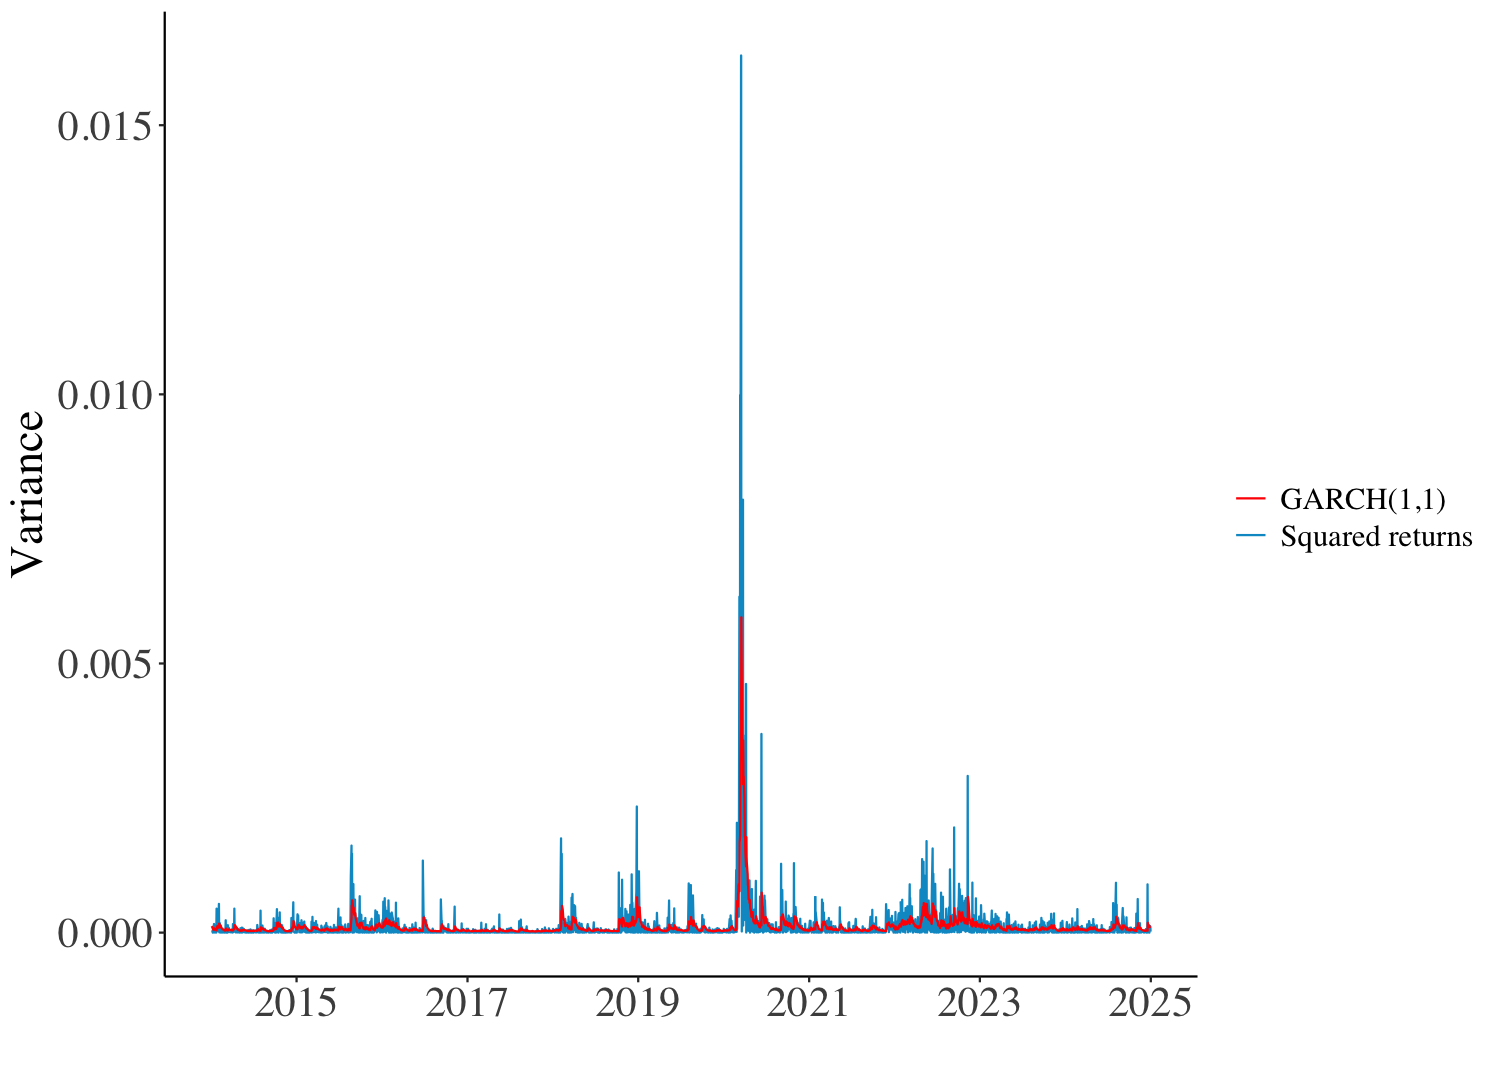
\includegraphics[scale=0.16]{../../plots/2.2.png} % Replace 
    \caption{Squared S\&P 500 returns with GARCH(1,1) variance parameters estimated using
QMLE.}
    \label{2.2}
\end{figure}


\begin{figure}[H]
    \centering
    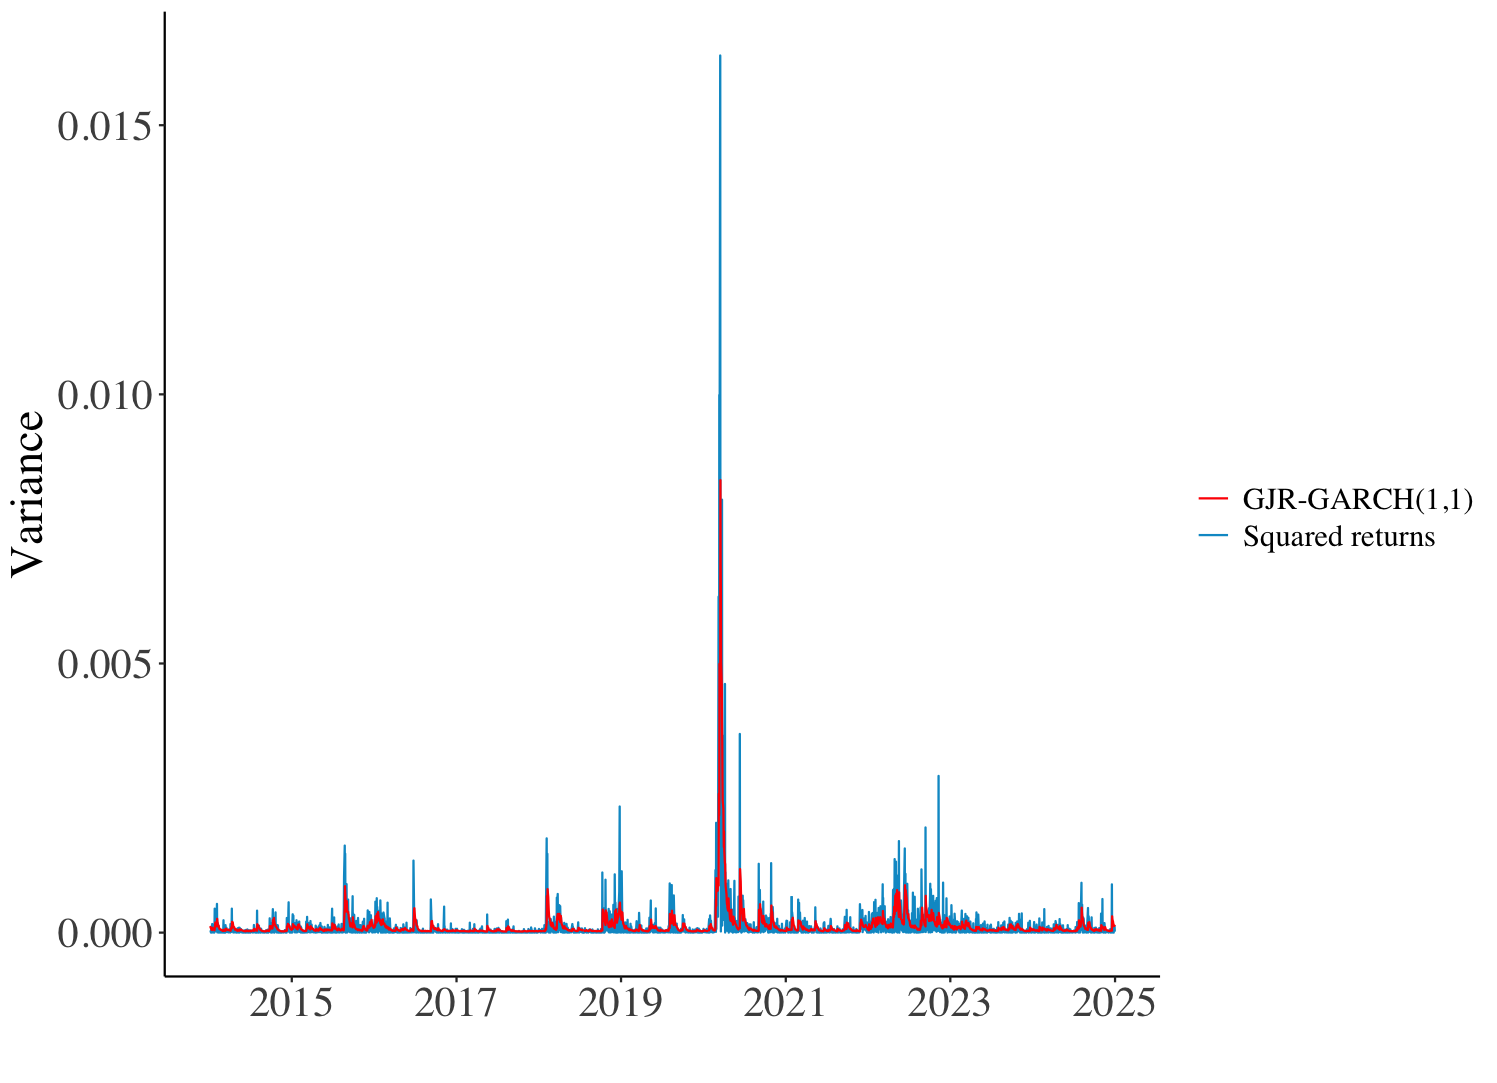
\includegraphics[scale=0.165]{../../plots/2.3.png} % Replace 
    \caption{Squared S\&P 500 returns with GJR-GARCH(1,1) variance parameters estimated using
QMLE.}
    \label{2.3}
\end{figure}

GARCH models possess several desirable theoretical properties that have been studied extensively, including the existence of a long-run variance and the ability to produce longer-horizon forecasts—features that may be relevant for risk management applications. In this chapter, we focus on daily returns and daily volatility forecasts.

Observe that $\alpha+\beta \approx 1$ in the fitted GARCH(1,1), and $\alpha+\beta+\alpha\theta\,\mathbb{E}[I_t]\approx1$ in the GJR–GARCH(1,1); under symmetric innovations $\mathbb{E}[I_t]=\tfrac{1}{2}$, giving $\alpha+\beta+\tfrac{1}{2}\alpha\theta \approx 1$. This near-unit persistence is common in financial return series \cite{Christoffersen2012}. When the persistence parameter equals one, i.e.\ $\alpha+\beta=1$ for GARCH(1,1) and $\alpha+\beta+\alpha\theta\,\mathbb{E}[I_t]=1$ for GJR–GARCH(1,1), the variance dynamics have a unit root (the IGARCH model case): the unconditional variance is not finite and multi-step variance forecasts do not mean-revert to a constant long-run level. As noted by \citeA{Tsay2010}, $\{\sigma_t^2\}$ is a martingale\footnote{A stochastic process \(\{X_t\}\) is a martingale with respect to an information set \(\{\mathcal{F}_t\}\) if its conditional expectation satisfies \(\mathbb{E}[X_{t+1}\mid\mathcal{F}_t]=X_t\). Intuitively, given current information, the best forecast of tomorrow’s value is today’s value.} in this setting, and the sources of volatility persistence warrant careful investigation.

Another important theoretical feature of GARCH models is their ability to generate return distributions with heavier tails than the normal distribution, even when normality is assumed for $z_{t+1}$. This means the volatility model itself contributes to capturing the excess kurtosis commonly observed in financial returns. \citeA{Bai2003} derive the kurtosis of GARCH models and show that, provided the kurtosis exists, the distribution of returns under a GARCH process can indeed exhibit heavier tails than the normal distribution.

Having analyzed return volatility, the next step is to properly model $z_{t+1}$, the standardized return or shock—keeping in mind the ultimate goal: to capture and replicate the empirical behavior of returns. The evaluation of the volatility models will be deferred to \hyperref[chap:4]{Chapter 4}, once the complete model for the return $R_{t+1}$ has been specified.
\newpage